\documentclass[12pt]{ximera}

\usepackage{nopageno}
\usepackage{amsmath}
\usepackage{graphicx}
\usepackage{geometry}
\geometry{top=1in,bottom=1in,right=0.75in,left=0.75in}
\usetikzlibrary{patterns}

\usepackage{fancyhdr}
\usepackage{lastpage}
 
\pagestyle{fancy}
\fancyhf{}
\rhead{\textsf{Form B}}
\lhead{\textsf{Calculus Knowledge Assessment v3}}
\rfoot{\textsf{Page \thepage\ of \pageref{LastPage}}}


\usepackage{multicol}
\setlength{\columnsep}{2cm}

\usepackage{enumitem}

\setitemize{noitemsep,topsep=0pt,parsep=0pt,partopsep=0pt}

\renewenvironment{multipleChoice}
{\begin{trivlist}\item[\hskip\labelsep\small\bfseries Choose the best answer:]
\hfil\begin{enumerate}\begin{multicols}{2}}
 {\end{multicols}\end{enumerate}\end{trivlist}}

\def\image{\begin{center}}
\def\endimage{\end{center}}

%\renewcommand{\choice}[2][]{\item \begin{minipage}[t]{2in}#2\end{minipage}\ifthenelse{\boolean{#1}}{\ifhandout \else \quad\checkmark\fi}{}}
\renewcommand{\choice}[2][]{\item \begin{minipage}[t]{2in}#2\end{minipage}\ifthenelse{\boolean{#1}}{\ifhandout \else  \fi}{}}


\begin{document}
\vspace{6ex}

\begin{minipage}{\textwidth}
\begin{problem}

  Four equally spaced numbers are shown below on a number line.
  \begin{image}
    \begin{tikzpicture}[x=0.19\textwidth]
      \draw[-{>[scale=1.75]}] (-0.05\textwidth,0) -- (0.8\textwidth,0);
      \foreach \x in {0,...,4} {%
        \draw (\x,-.1) -- (\x,.1);
        \node[anchor=north,yshift=-2pt] at (\x,0) {$\x$};
      }
      \draw (0.5,0) node [circle,fill,inner sep=1pt,label=above:$x$](e){};
      \draw (1.5,0) node [circle,fill,inner sep=1pt,label=above:$y$](e){};
      \draw (2.5,0) node [circle,fill,inner sep=1pt,label=above:$z$](e){};
      \draw (3.5,0) node [circle,fill,inner sep=1pt,label=above:$w$](e){};
    \end{tikzpicture}
  \end{image}
  Let $f(t) = t^2$ and consider $f(x)$ and $f(y)$ and $f(z)$ and $f(w)$.  Which pair of numbers is farthest apart?
  \begin{multipleChoice}
    \choice{The pair $f(x)$ and $f(y)$.}
    \choice{The pair $f(y)$ and $f(z)$.}
    \choice[correct]{The pair $f(z)$ and $f(w)$.}
    \choice{These pairs are all equally far apart}
  \end{multipleChoice}
\end{problem}
\end{minipage}

\vspace{6ex}

\begin{minipage}{\textwidth}
\begin{problem}
  The graph below is a plot of a function $f$.  What best describes
  the behavior of $f$ on the interval from $x=-2$ to $x=2$?
  \begin{image}
    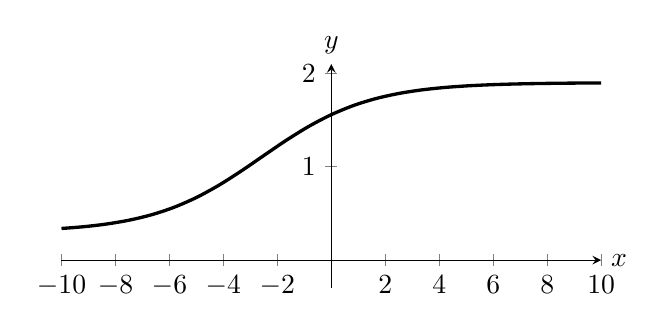
\begin{tikzpicture}
      \begin{axis}[
        clip=false,
        y post scale=0.5,
        domain=-10:10, 
        ytickmin=0,ytickmax=3,
        ytick={1,2},
        xtickmin=-10,xtickmax=10,
        xtick={-10,-8,-6,-4,-2,2,4,6,8,10},
        ymin=-0.3, ymax=2.1,
        xlabel=$x$, ylabel=$y$,
        axis lines=center,
        every axis y label/.style={at=(current axis.above origin),anchor=south},
        every axis x label/.style={at=(current axis.right of origin),anchor=west},
        axis on top,
        ]          
        \addplot [very thick,smooth] {0.3 + 1.6/(1 + exp(-0.5*(x + 2.6))};
      \end{axis}
    \end{tikzpicture}
    \end{image}
  \begin{multipleChoice}
    \choice{As $x$ increases, $f(x)$ is increasing at an increasing rate.}
    \choice[correct]{As $x$ increases, $f(x)$ is increasing at a decreasing rate.}
    \choice{As $x$ increases, $f(x)$ is increasing at a constant rate.}
    \choice{As $x$ increases, $f(x)$ is decreasing at a decreasing rate.}
    \choice{As $x$ increases, $f(x)$ is decreasing at an increasing rate.}
  \end{multipleChoice}
\end{problem}
\end{minipage}

\vspace{6ex}

\begin{minipage}{\textwidth}
\begin{problem} 

  Pick two numbers positve real numbers $a$ and $b$ so that
  $a \approx b$.  Pick a very large integer $N$.  What can you say
  about $a^N$ and $b^N$?
  \begin{multipleChoice}
    \choice{$a^N$ and $b^N$ must both be large because $N$ is large.}
    \choice{$a^N$ and $b^N$ must both be small because $|a-b|^N$ is small.}
    \choice{$a^N$ must be very close to $b^N$ because $a \approx b$.}
    \choice[correct]{$a^N$ might not be very close to $b^N$ even though $a \approx b$.}
  \end{multipleChoice}
\end{problem}
\end{minipage}

\vspace{6ex}

\begin{minipage}{\textwidth}
\begin{problem}

  Suppose $f$ is an increasing function and $f(x) + g(x)$ is a constant.  How does $g$ depend on $x$?
  \begin{multipleChoice}
    \choice{$g$ must be increasing.}
    \choice{$g$ could be constant.}
    \choice[correct]{$g$ must be decreasing.}
    \choice{None of the above.}
  \end{multipleChoice}
\end{problem}
\end{minipage}

\vspace{6ex}

\begin{minipage}{\textwidth}
\begin{problem}

  Suppose $f$ and $g$ are increasing functions with domain consisting of all real numbers.  What can be said about the function $h(x) = f(g(x))$?
  \begin{multipleChoice}
    \choice{It is a decreasing function.}
    \choice{It is a constant function.}
    \choice[correct]{It is an increasing function.}
    \choice{It depends on exactly which functions $f$ and $g$ are being considered.}
  \end{multipleChoice}
\end{problem}
\end{minipage}

\vspace{6ex}

\begin{minipage}{\textwidth}
\begin{problem}
  Suppose $f$ is a differentiable function and $f(0) = 0$ and
  $f(\sin 0.03) = 6$.  What is a best guess for $f(0.01)$?
  \begin{multipleChoice}
    \choice[correct]{$2$}
    \choice{$4$}
    \choice{$6$}
  \end{multipleChoice}
\end{problem}
\end{minipage}

\vspace{6ex}

\begin{minipage}{\textwidth}
\begin{problem}
  Suppose a polynomial $f$ achieves a global minimum, and besides that
  one point has no other local or global extrema.  What must be true
  of $f$?
  \begin{multipleChoice}
    \choice{$f'$ is a constant function}
    \choice{$f''$ is a constant function but it could be either negative or positive}
    \choice{$f''$ is a constant function and must be positive}
    \choice[correct]{None of these statements are true.}
  \end{multipleChoice}
\end{problem}
\end{minipage}

\vspace{6ex}

\begin{minipage}{\textwidth}
\begin{problem}
  Two pairs of numbers are shown below.
  \begin{image}
    \begin{tikzpicture}[x=0.19\textwidth]
      \draw[-{>[scale=1.75]}] (-0.05\textwidth,0) -- (0.8\textwidth,0);
      \foreach \x in {0,...,4} {%
        \draw (\x,-.1) -- (\x,.1);
        \node[anchor=north,yshift=-2pt] at (\x,0) {$\x$};
      }
      \draw (0.25,0) node [circle,fill,inner sep=1pt,label=above:$s$](e){};
      \draw (1.25,0) node [circle,fill,inner sep=1pt,label=above:$s+h$](e){};
      \draw (2.75,0) node [circle,fill,inner sep=1pt,label=above:$t$](e){};
      \draw (3.75,0) node [circle,fill,inner sep=1pt,label=above:$t+h$](e){};
    \end{tikzpicture}
  \end{image}
  Let $f(x) = -1/x$.  How does $f(s+h)-f(s)$ compare with $f(t+h) - f(t)$?
  \begin{multipleChoice}
    \choice{$f(s+h) - f(s) < f(t+h) - f(t)$}
    \choice{$f(s+h) - f(s) = f(t+h) - f(t)$}
    \choice[correct]{$f(s+h) - f(s) > f(t+h) - f(t)$}
  \end{multipleChoice}
\end{problem}
\end{minipage}

\vspace{6ex}

\begin{minipage}{\textwidth}
\begin{problem}
  Suppose $f$ is a function (with domain consisting of nonzero real numbers) so that $f'(x) = 1/x$.  What must be true of $f$?
  \begin{multipleChoice}
    \choice{$f(x) = \ln x$}
    \choice{$f(x) = \ln |x|$}
    \choice{There is a number $C$ (possibly zero) so that $f(x) = C + \ln x$}
    \choice{There is a number $C$ (possibly zero) so that $f(x) = C + \ln |x|$}
    \choice[correct]{$\frac{d}{dx} \left( f(x) - \ln |x| \right) = 0$}
  \end{multipleChoice}
\end{problem}
\end{minipage}

\vspace{6ex}

\begin{minipage}{\textwidth}
\begin{problem}
  Two pairs of numbers are shown below.
  \begin{image}
    \begin{tikzpicture}[x=0.19\textwidth]
      \draw[-{>[scale=1.75]}] (-0.05\textwidth,0) -- (0.8\textwidth,0);
      \foreach \x in {0,...,4} {%
        \draw (\x,-.1) -- (\x,.1);
        \node[anchor=north,yshift=-2pt] at (\x,0) {$\x$};
      }
      \draw (3.141592654,-.1) -- (3.141592654,.1);
      \node[anchor=north,yshift=-2pt] at (3.141592654,0) {$\pi$};
      \draw (0.25,0) node [circle,fill,inner sep=1pt,label=above:$s$](e){};
      \draw (0.65,0) node [circle,fill,inner sep=1pt,label=above:$s+h$](e){};
      \draw (3.19,0) node [circle,fill,inner sep=1pt,label=above:$t$](e){};
      \draw (3.59,0) node [circle,fill,inner sep=1pt,label=above:$t+h$](e){};
    \end{tikzpicture}
  \end{image}
  Let $f(x) = \sin x$.  How does $f(s+h)-f(s)$ compare with $f(t+h) - f(t)$?
  \begin{multipleChoice}
    \choice{$f(s+h) - f(s) < f(t+h) - f(t)$}
    \choice{$f(s+h) - f(s) = f(t+h) - f(t)$}
    \choice[correct]{$f(s+h) - f(s) > f(t+h) - f(t)$}
  \end{multipleChoice}
\end{problem}
\end{minipage}

\vspace{6ex}

\begin{minipage}{\textwidth}
\begin{problem}
  Suppose $f(x) = x^2$.  How does $f(f(x))$ compare to $f(x)$?
  \begin{multipleChoice}
    \choice{Whenever $x$ is close to one, $f(f(x))$ is close to zero.}
    \choice{Whenever $x$ is close to one, $f(f(x))$ is larger than $x$.}
    \choice{Whenever $x$ is close to zero, $f(f(x))$ is larger than $x$.}
    \choice[correct]{Whenever $x$ is large, $f(f(x))$ is larger than $x$.}
  \end{multipleChoice}
\end{problem}
\end{minipage}

\vspace{6ex}

\begin{minipage}{\textwidth}
\begin{problem}
  Suppose $f(a)$ is the area of the region bounded by $x^2 + y^2 \leq 25$ and $-5 \leq x \leq a$.  What integer is closest to $\frac{f(4.01) - f(4)}{0.01}$?
  \begin{multipleChoice}
    \choice{3}
    \choice{4}
    \choice{5}
    \choice[correct]{6}
  \end{multipleChoice}
\end{problem}
\end{minipage}

\vspace{6ex}

\begin{minipage}{\textwidth}
\begin{problem}
  Suppose $f$ is a continuous function.  Consider $g(n) = \int_0^1 f(x^n) \, dx$.  When $n$ is very large, what is a good guess as to the value of $g(n)$?
  \begin{multipleChoice}
    \choice[correct]{When $n$ is large, $g(n)$ is close to $f(0)$}
    \choice{When $n$ is large, $g(n)$ is close to $f(1)$}
    \choice{When $n$ is large, $g(n)$ is close to the average value of $f$ on the interval $[0,1]$}
  \end{multipleChoice}
\end{problem}
\end{minipage}

\vspace{6ex}

\begin{minipage}{\textwidth}
\begin{problem}
  Consider the function $f(x) = e^x - x$.  What must be true about $f$?
  \begin{multipleChoice}
    \choice[correct]{$f(x) \geq 1$ for all $x$}
    \choice{$f(x) \leq 1$ for all $x$}
  \end{multipleChoice}
\end{problem}
\end{minipage}

\vspace{6ex}

\begin{minipage}{\textwidth}
\begin{problem}
	Let $f$ be the function defined by $f(x) = x^2+1$, and $g$ be the function defined by the rule $g(z) = z^2+1$. 
	\begin{multipleChoice}
		\choice{Since $f$ and $g$ have differing domain, they are different functions}
		\choice[correct]{$f$ and $g$ are the same function}
		\choice{$f$ and $g$ are different functions because they disagree for some inputs in their common domain}
		\choice{$f$ and $g$ are different functions because they are of different variables}
	\end{multipleChoice}
\end{problem}
\end{minipage}

\vspace{6ex}

\begin{minipage}{\textwidth}
\begin{problem}
  The expression $\log_b(x) = y$ is equivalent to:
  \begin{multipleChoice}
    \choice{$b^x = y$}
    \choice[correct]{$b^y = x$}
    \choice{$x^b = y$}
    \choice{$x^y = b$}
    \choice{$y^b = x$}
    \choice{$y^x = b$}
  \end{multipleChoice}  
\end{problem}
\end{minipage}

\vspace{6ex}

\begin{minipage}{\textwidth}
\begin{problem}
	Suppose $x$ is a small negative number.  What can be said about $\frac{x}{|x|}$?
	\begin{multipleChoice}
		\choice[correct]{It is close to $-1$}
		\choice{It is close to $1$}
		\choice{It is close to $0$}
	\end{multipleChoice}
\end{problem}
\end{minipage}

\vspace{6ex}

\begin{minipage}{\textwidth}
\begin{problem}
  Suppose $A$ and $a$ differ by at most $2$ and suppose $B$ and $b$
  differ by at most $1$.  In symbols, this means that $|A - a| < 2$ and $|B - b| < 1$.
  By how much could $A/B$ and $a/b$ differ?
  \begin{multipleChoice}
    \choice{By no more than $1$, meaning $|A/B - a/b| < 1$}
    \choice{By no more than $2$, meaning $|A/B - a/b| < 2$}
    \choice{By no more than a factor of $2$, meaning $\left| \frac{A/B}{a/b} \right| < 2$}
    \choice{By no more than a factor of $1/2$, meaning $\left| \frac{A/B}{a/b} \right| < \frac{1}{2}$}
    \choice[correct]{By any amount}
  \end{multipleChoice}
\end{problem}
\end{minipage}

\vspace{6ex}

\begin{minipage}{\textwidth}
\begin{problem}
  Pick two numbers $a$ and $b$ in the interval $[0,1]$ so that
  $a \approx b$.  Pick a very large integer $N$.  How does $a^N$
  compare to $b^N$?
  \begin{multipleChoice}
    \choice{$a^N$ is very close to $b^N$ because $a \approx b$}
    \choice[correct]{$a^N$ need not be very close to $b^N$ even though $a \approx b$}
  \end{multipleChoice}
\end{problem}
\end{minipage}

\vspace{6ex}

\begin{minipage}{\textwidth}
\begin{problem}
  Let $f(x) = x^{800}$.  How does $A = f(10^{10} + 1) - f(10^{10})$ compare to $B = f(10^{10}) - f(10^{10} - 1)$?
  \begin{multipleChoice}
    \choice{$A < B$}
    \choice{$A = B$}
    \choice[correct]{$A > B$}
  \end{multipleChoice}
\end{problem}
\end{minipage}

\end{document}

%%% Local Variables:
%%% mode: latex
%%% TeX-master: t
%%% End:
